%!TEX root = Nanomat.tex
\ctitle{Å lage tynnfilmer med CVD og PVD}
I dette kapittelet fortsetter vi å lage tynnfilmer, men i dette tilfellet er forløperne til tynnfilmen i ``dampfase'' (vapor-phase). I \emph{Chemical Vapor Deposition (CVD)} har vi en damp av molekyler, og i \emph{Physical Vapor Deposition (PVD)} har vi en damp av atomer.

\paragraph{Generelle ting å tenke på}
Kontroller substrattemperatur og deponeringstemperatur, hold dem så lave som mulig (for å gjøre dette bruker vi gjerne plasma - plasma sørger for høy mobilitet og reaktivitet selv ved lave temperaturer). Dette for å hindre ukontrollert kornvekst og diffusjon mellom lag i flerlagsfilmer. 

\cstitle{Chemical Vapor Deposition (CVD)}
I CVD introduserer vi gasser i den ene enden av et kammer, lar disse gassene diffundere og reagere for å danne en tynnfilm på et substrat, og fjerner biprodukter fra den andre enden av kammeret. Den generelle flyten i CVD er beskrevet i figuren, men det finnes mange forskjellige varianter av CVD som på den ene eller den andre måten gjør prosessen mer effektiv.

\begin{figure}[H]
\bmd\centering
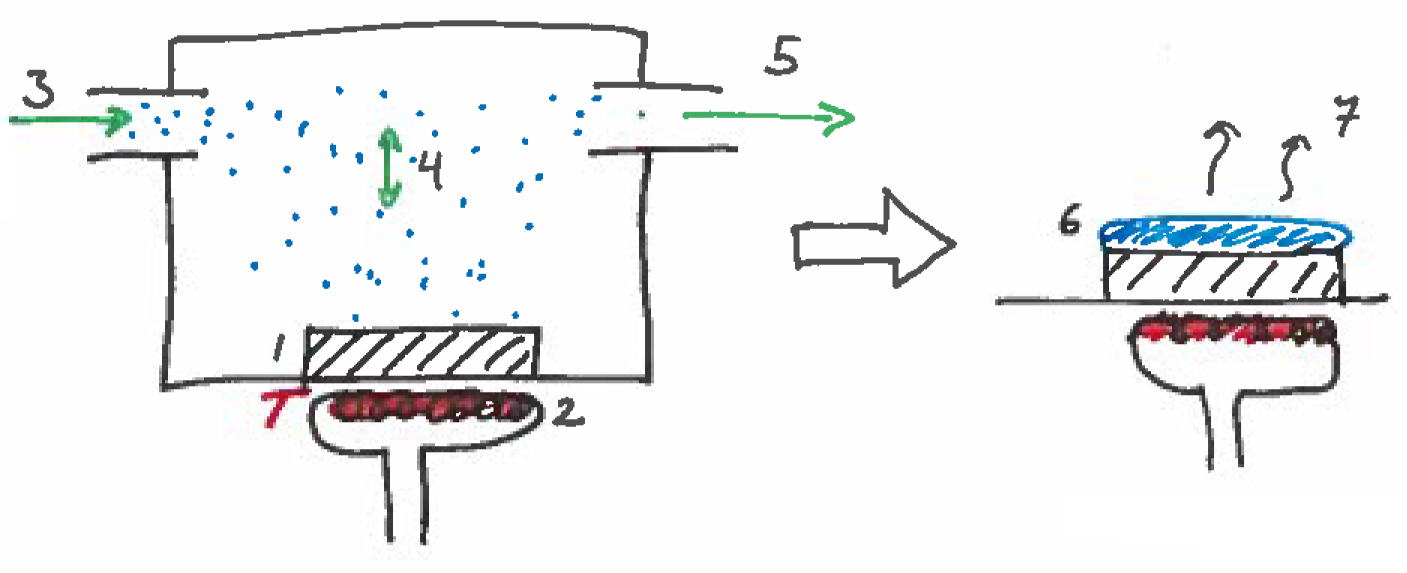
\includegraphics[width=\linewidth]{metodefigs/cvd.png}
\caption{Sånn kan man gjøre CVD. 1: Substrat. 2: Varme. 3: Gass med de kjemiske forløperne til filmen kommer inn i kammeret. 4: Gassen diffunderer på tvers av luftstrømmen. 5: Gassen pumpes ut av kammeret ved vakuum. 6: Overflatereaksjoner på substratet fører til at en film dannes. 7: Eventuelle biprodukter må vekk fra filmen.}
\emd\end{figure}

Gassene kan enten: reagere mens de er i ``lufta'', og så bli deponert på substratet; eller de kan vente med å reagere til de har landet på substratet. For å aktivere de kjemiske reaksjonene kan vi enten bruke varme, eller vi kan bruke plasma. Hvis vi bruker varme kalles det en \emph{termisk aktivert CVD-prosess}, og her kan vi velge mellom å bruke en ``hot-walled reactor'' (der hele reaktoren varmes opp) eller en ``cold-walled reactor'' (der kun substratet varmes opp). Temperaturen i termisk aktiverte CVD-prosesser er gjerne \SI{1200}{\kelvin} eller høyere. Hvis vi i stedet velger å bruke plasma til å aktivere reaksjonene, klarer vi oss med en lavere temperatur.

Noen av fordelene og ulempene med CVD:
\begin{itemize}
	\item Vi kan gro filmer med forholdsvis høy hastighet (noen mikrometer pr. time)
	\item Vi kan gro filmer som har uniform tykkelse, også hvis substratet har en meget funky form
	\item Gassene som brukes i CVD er ofte giftige eller farlige på andre måter
	\item Man kan lage alt mulig rart av tynnfilmer med CVD avhengig av hvilke gasser man introduserer i kammeret.
	\item Temperaturen i termisk aktiverte CVD-prosesser er upraktisk høy. Hvis vi bruker plasma (neste avsnitt) kan vi gjøre temperaturen mer levelig.
\end{itemize}
Før vi ser på plasma-aktivert CVD, må vi finne ut hvordan man lager plasma:

\paragraph{DIY guide: hvordan lage plasma} En vanlig måte å lage plasma på, er å putte en gass (for eksempel \ce{Ar}) i et kraftig elektrisk felt som alternerer med en frekvens på rundt \SI{13.56}{\mega\hertz} (som er i frekvensområdet til høyfrekvente radiobølger). Da vil elektronene på en måte ristes løs fra argonkjernen, fordi elektronet akselereres mye mer enn den tyngre argonkjernen.
\begin{figure}[H]
\bmd\centering
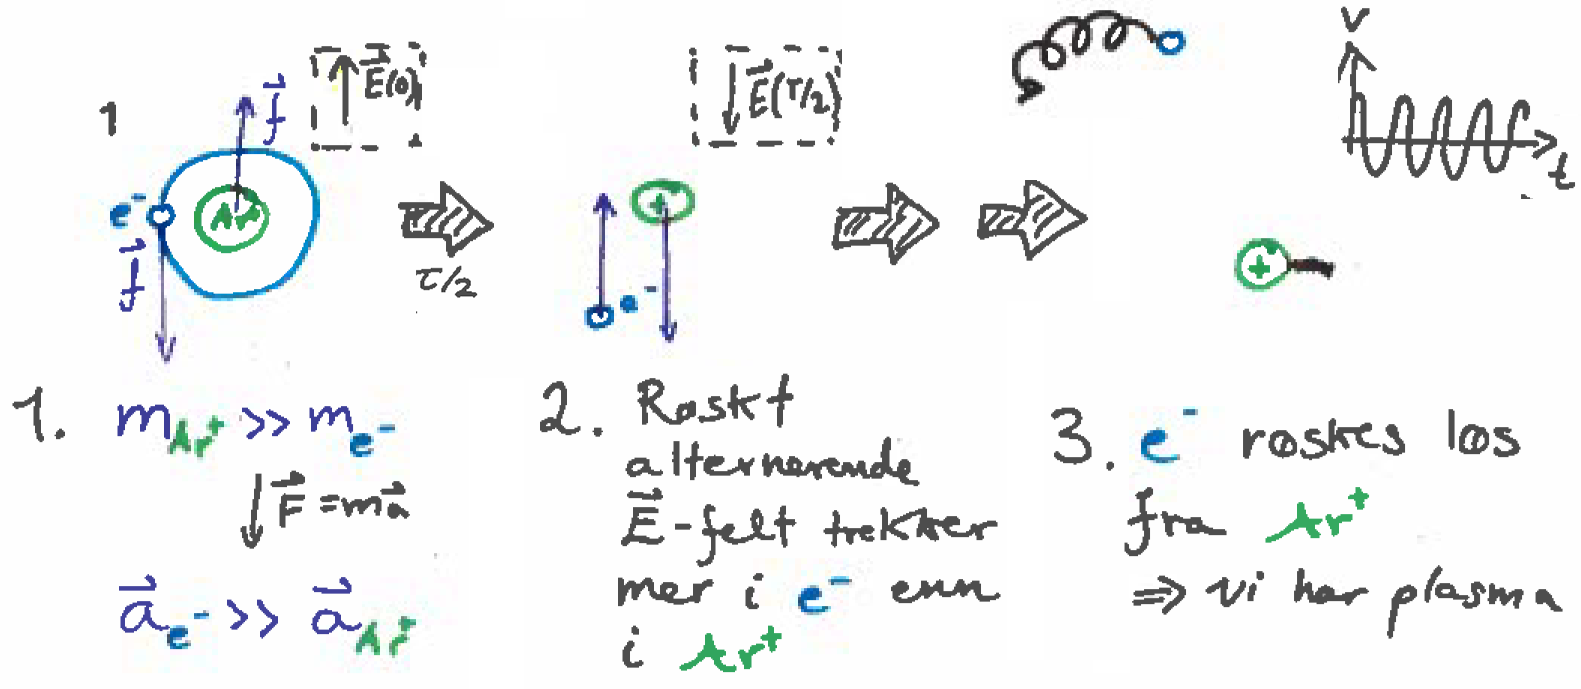
\includegraphics[width=\linewidth]{metodefigs/plasmagen.png}
\caption{Sånn kan man lage plasma. Bruk vernebriller!}
\emd\end{figure}

\paragraph{Plasma-enhanced CVD (PECVD)} I plasma-aktivert CVD lager vi plasma av gassene. De ioniserte gassene er veldig reaktive, og vi trenger derfor ikke den samme temperaturen for å oppnå reaksjonene som skal til for å lage en tynnfilm. Temperaturen er gjerne \SI{800}{\kelvin} eller lavere for PECVD.

En ytterligere fordel med PECVD er at man kan bruke et elektrisk felt til å akselerere reaktantene mot substratet, siden ionene har ladning. Dermed kan man få strukturer smo gror i én bestemt retning. Man kan for eksempel gro karbonnanorør som gror vertikalt (og ikke bare det -- man kan bestemme rollup-vektoren også!), noe som ville vært vanskelig med termisk aktivert CVD der ting gror isotropt.

\cstitle{Physical Vapor Deposition (PVD)}
PVD kort forklart: du har en blokk med materialet du vil lage tynnfilm av (denne blokken kalles ``target'' i PVD-sammenheng). Du tilfører dette kildematerialet en god bunt med energi. Energien gjør at atomer løsner fra kildematerialet. Disse atomene fanger du opp med substratet. Denne prosessen involverer som regel ikke kjemiske reaksjoner.

\paragraph{Evaporation-PVD} I evaporation-PVD tilfører du energien i form av varme:
\begin{figure}[H]
\bmd\centering
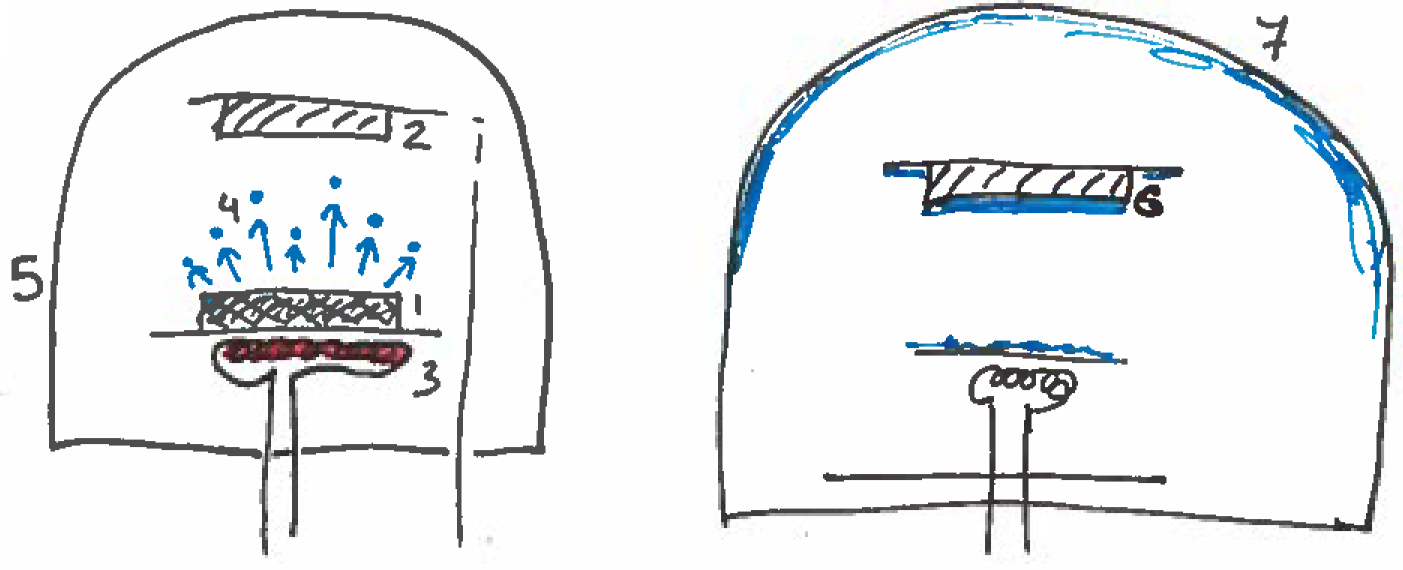
\includegraphics[width=\linewidth]{metodefigs/evappvd.png}
\caption{Sånn kan man gjøre evaporation-PVD. 1: Kilde til materialet (``target''). 2: Substrat. 3: Resistiv oppvarming av target. 4. Atomer fra kildematerialet løsner fra target ved fordamping. 5. Alt skjer inne i et vakuumkammer med trykk mellom $10^{-3}$ og $10^{-10}$ torr. 6: En film dannes på substratet. 7: En film dannes også overalt eller på utstyret :(}
\emd\end{figure}
Hvis du bare tilfører varme vil atomene fare overalt etter at de har løsnet, så hele PVD-systemet kommer til å bli dekket med tynnfilm hvis du bruker denne metoden. Det samme gjelder mange typer PVD.

\paragraph{Molecular Beam Epitaxy} er en mer fancy og sammensatt variant av evaporation-PVD, der man har flere \emph{Knudsen-celler} med hver sin blokk av kildemateriale som varmes opp på samme måte som i evaporation-PVD. MBE kjennetegnes ved et \emph{ultrahøyt vakuum}, og at atomene eller molekylene fra kildematerialet ikke interagerer med hverandre. Vekst-mekanismen i MBE blir dermed meget enkel og lett å kontrollere. Veksten skjer atomlag for atomlag, og går dermed temmelig sakte -- hastigheten til veksten er mindre enn en mikrometer i timen. Siden tynnfilmvekst med MBE er treig og kontrollerbar, brukes den til å lage tynnfilmer som er énkrystaller. Man kan også lage multikrystalline filmer med skarpe grenseflater mellom hvert lag av filmen (se figur).
\begin{figure}[H]
\bmd\centering
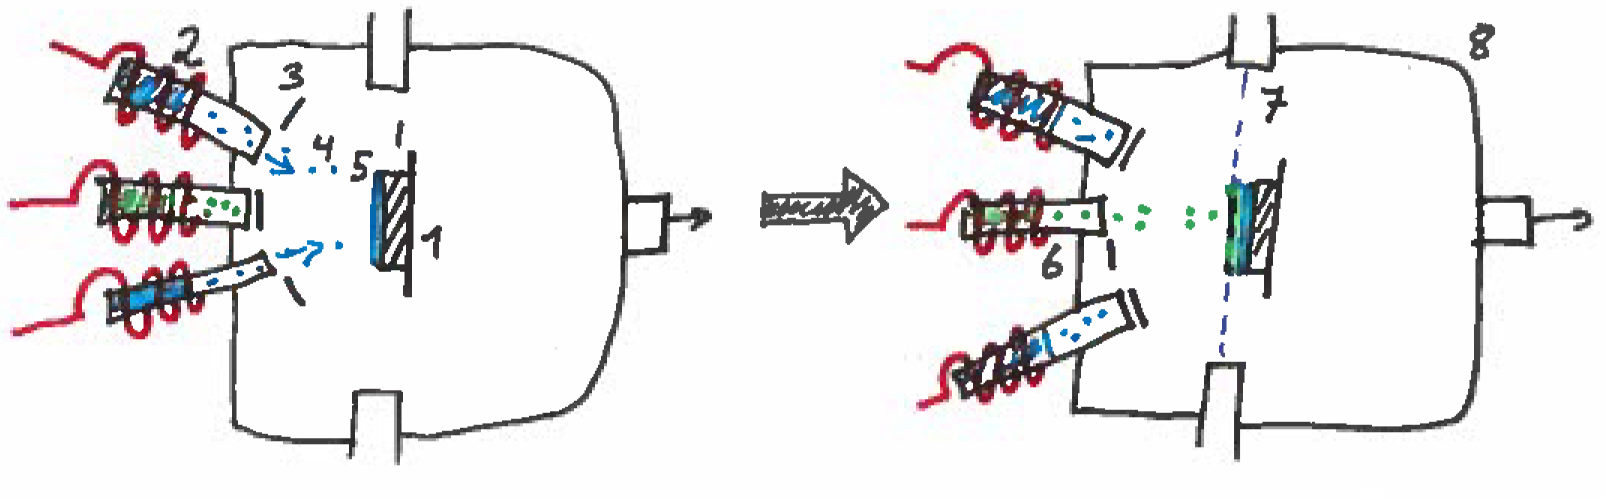
\includegraphics[width=\linewidth]{metodefigs/mbe.png}
\caption{Sånn kan man gjøre MBE. 1: Substrat. 2: Knudsen-celler -- kildematerialet varmes opp og fordamper her. 3/4: Lukkere åpner og lukkes for å kontrollere hva som når frem til substratet. 5: Det som når fram til substratet, danner en film der. 6: Bytt mellom hvilke lukkere som er åpne for å gro lagvise filmer. 7: Mulighet for \emph{in situ}-karakterisering (for eksempel RHEED). 8: vakumkammer med ultrahøyt vakuum er nødvendig i MBE.}
\emd\end{figure}
En fordel med MBE er at det er (relativt) lett å putte inn måleinstrumenter som karakteriserer materialet \emph{in situ} mens det gror. Dette gir enda bedre muligheter for å kontrollere prosessen.

\paragraph{Elektronstråle-PVD} I elektronstråle-PVD (electron beam PVD, EBPVD) er det en stråle av høyenergetiske elektroner som er energikilden. Siden elektronstrålen kan fokuseres, er det mulig å bruke materialet mer effektivt enn med andre metoder. I tillegg trenger ikke temperaturen å være særlig høy. Deponeringsraten med EBPVD er ganske høy, mellom ca. 0.1 og 100 mikrometer i \emph{minuttet}. 

I tillegg til elektronstrålen kan man bruke ionekilder til å modifisere substratet (dette gjøres \emph{etter} at elektronstrålen har blitt brukt). Dette kalles \emph{ionestråle-assistert} EBPVD. Ionestrålen kan brukes direkte til å etche eller rense substratet, kontrollere mikrostrukturen til substratet, eller til å modifisere filmen etter at den er deponert.

\paragraph{Sputtering} I sputtering bombarderes target med ioner, som gjør at atomer fra target løsner, og så treffer de substratet. Enkelt og greit.
\begin{figure}[H]
\bmd\centering
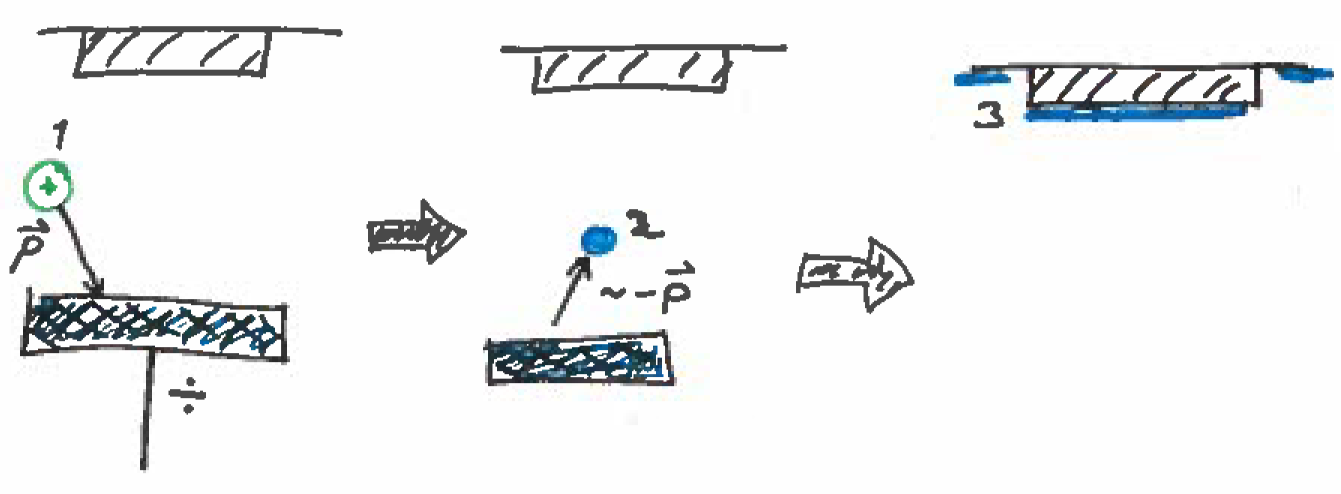
\includegraphics[width=\linewidth]{metodefigs/sputring.png}
\caption{Sputtering. 1. Argonioner fra plasma treffer target. 2: Atomer fra kilden løsner... 3: ...og dekker substratet (samt resten av utstyret) med en film.}
\emd\end{figure}

\paragraph{Cathodic sputtering} I katodisk sputring lar man target være en katode (altså holdes den ved et negativt potensial), slik at de positive ionene akselereres mot target. Dette slår løs nøytrale atomer fra target, og disse nøytrale atomene kan uten problemer komme seg på tvers av det elektriske feltet og frem til substratet.

\paragraph{Magnetron sputtering} Magnetron sputtering er en forbedring av katodisk sputring der man bruker magneter til å holde elektronene nær overflaten av target. Dette fører til høyere plasmatetthet i området rundt target,\footnote{Mulig forklaring: det er litt som hvordan radiofrekvente alternerende felt lager plasma ved at argonionene ikke klarer å holde følge med elektronene --- i dette tilfellet blir det at de magnetiske feltlinjene er sterke nok til å holde elektronene i nærheten av target, men ikke sterke nok til å holde argonionene i nærheten av target.} og det gjør også at ionene har høyere energi. Dermed for også de sputrede atomene høyere energi, slik at den resulterende filmen blir tettere og sitter bedre fast i substratet.

\paragraph{Ion beam sputtering} Med denne metoden dropper man plasma og felt og sånn, og bare skyter en ionestråle rett på target. Fordelen med denne metoden er at man kan kontrollere energien til ionene bedre (den avhenger kun av forholdene i ionestråle-generatoren), man kan ha både høy ionetetthet og en tykk stråle, og man kan gjøre deponeringen under et høyere vakuum enn man kan i plasmasputtering (som er fint hvis man av andre grunner trenger høyt vakuum).

\paragraph{Pulsed Laser Deposition (PLD)} I PLD er det ikke energetiske ioner, men en energetisk laser som treffer substratet.
\begin{figure}[H]
\bmd\centering
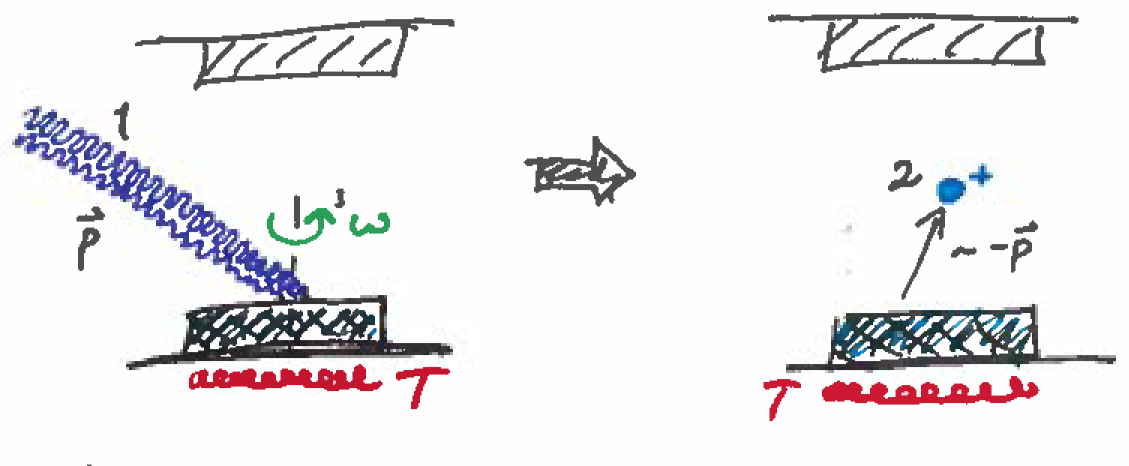
\includegraphics[width=\linewidth]{metodefigs/pld.png}
\caption{Pulsed Laser Deposition. 1: Laser treffer kilden, og feltet i laseren er nok til å røske elektronene løs fra materialet. 2: Ionisert materiale fordamper ved oppvarming. 3: Kilden kan roteres for å beskytte materialet, eller for å variere hvilket stoff som deponeres.}
\emd\end{figure}

\paragraph{Cathodic arc evaporation} I cathodic arc evaporation lager man et veldig sterkt elektrisk felt mellom target og en anode. Dette fører til en voldsom lokal temperaturøkning som gjør at materialet evaporerer her.
\begin{figure}[H]
\bmd\centering
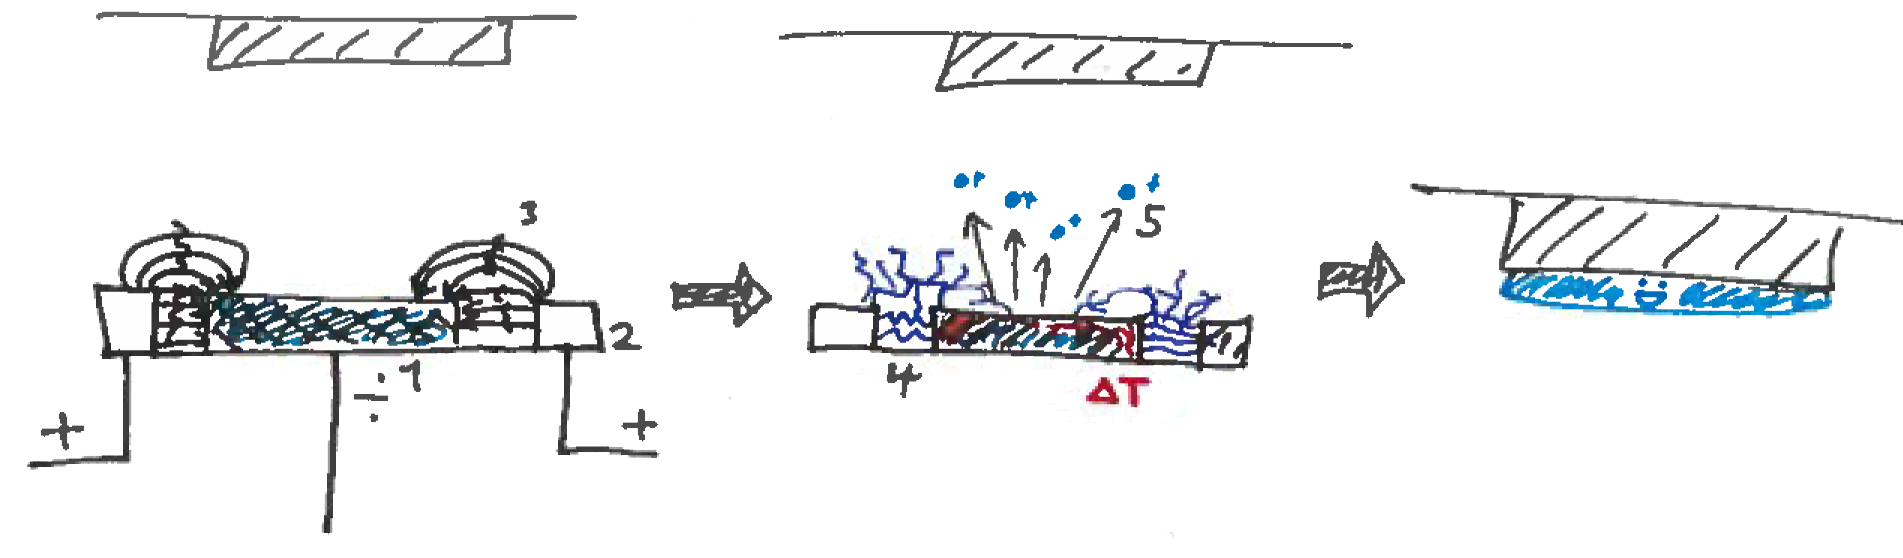
\includegraphics[width=\linewidth]{metodefigs/arcdep.png}
\caption{Cathodic arc sputtering. 1: Kilden er én elektrode. 2: Rett ved siden av kilden har man motsatt elektrode. 3: Det dannes et veldig stort lokalt $E$-felt. 4. Gjennomslag (dannelse av en lysbue) og temperaturøkning. 5: Materialet ioniseres (på grunn av lysbuen) og fordamper (på grunn av temperaturøkningen).}
\emd\end{figure}